\documentclass{../../../../style/mkimain}

\series{1}
\month{únor}
\year{2023}

\begin{document}
\section*{I.U1 Slavné osobnosti fyziky}
\noindent K obrázkům níže přiřaďte jména vyobrazených fyziků a jejich přínos vědě (využijte pojmy z následujích rámečků).
\\
\begin{mdframed}[frametitle={Jména}, frametitlealignment=\center, innerbottommargin=5px]
    \begin{center}
        Albert~Einstein, Isaac~Newton, Michael~Faraday, Stephen~Hawking, Erwin~Schrödinger, Marie~Curie-Skłodowska
    \end{center}
\end{mdframed}
\vspace{0.5cm}
\begin{mdframed}[frametitle={Díla}, frametitlealignment=\center, innerbottommargin=5px]
    \begin{center}
        speciální~princip~relativity, gravitační~zákon, elektromagnetická~indukce, stanovení~teploty~černé~díry, myšlenkový~experiment~s~kočkou~v~krabici, teorie~radioaktivity
    \end{center}
\end{mdframed}
\proborigin{Vojta hledá inspiraci na SOČ}
\klein
\begin{figure}[H]
  \minipage{0,3\textwidth}
  \begin{center}
    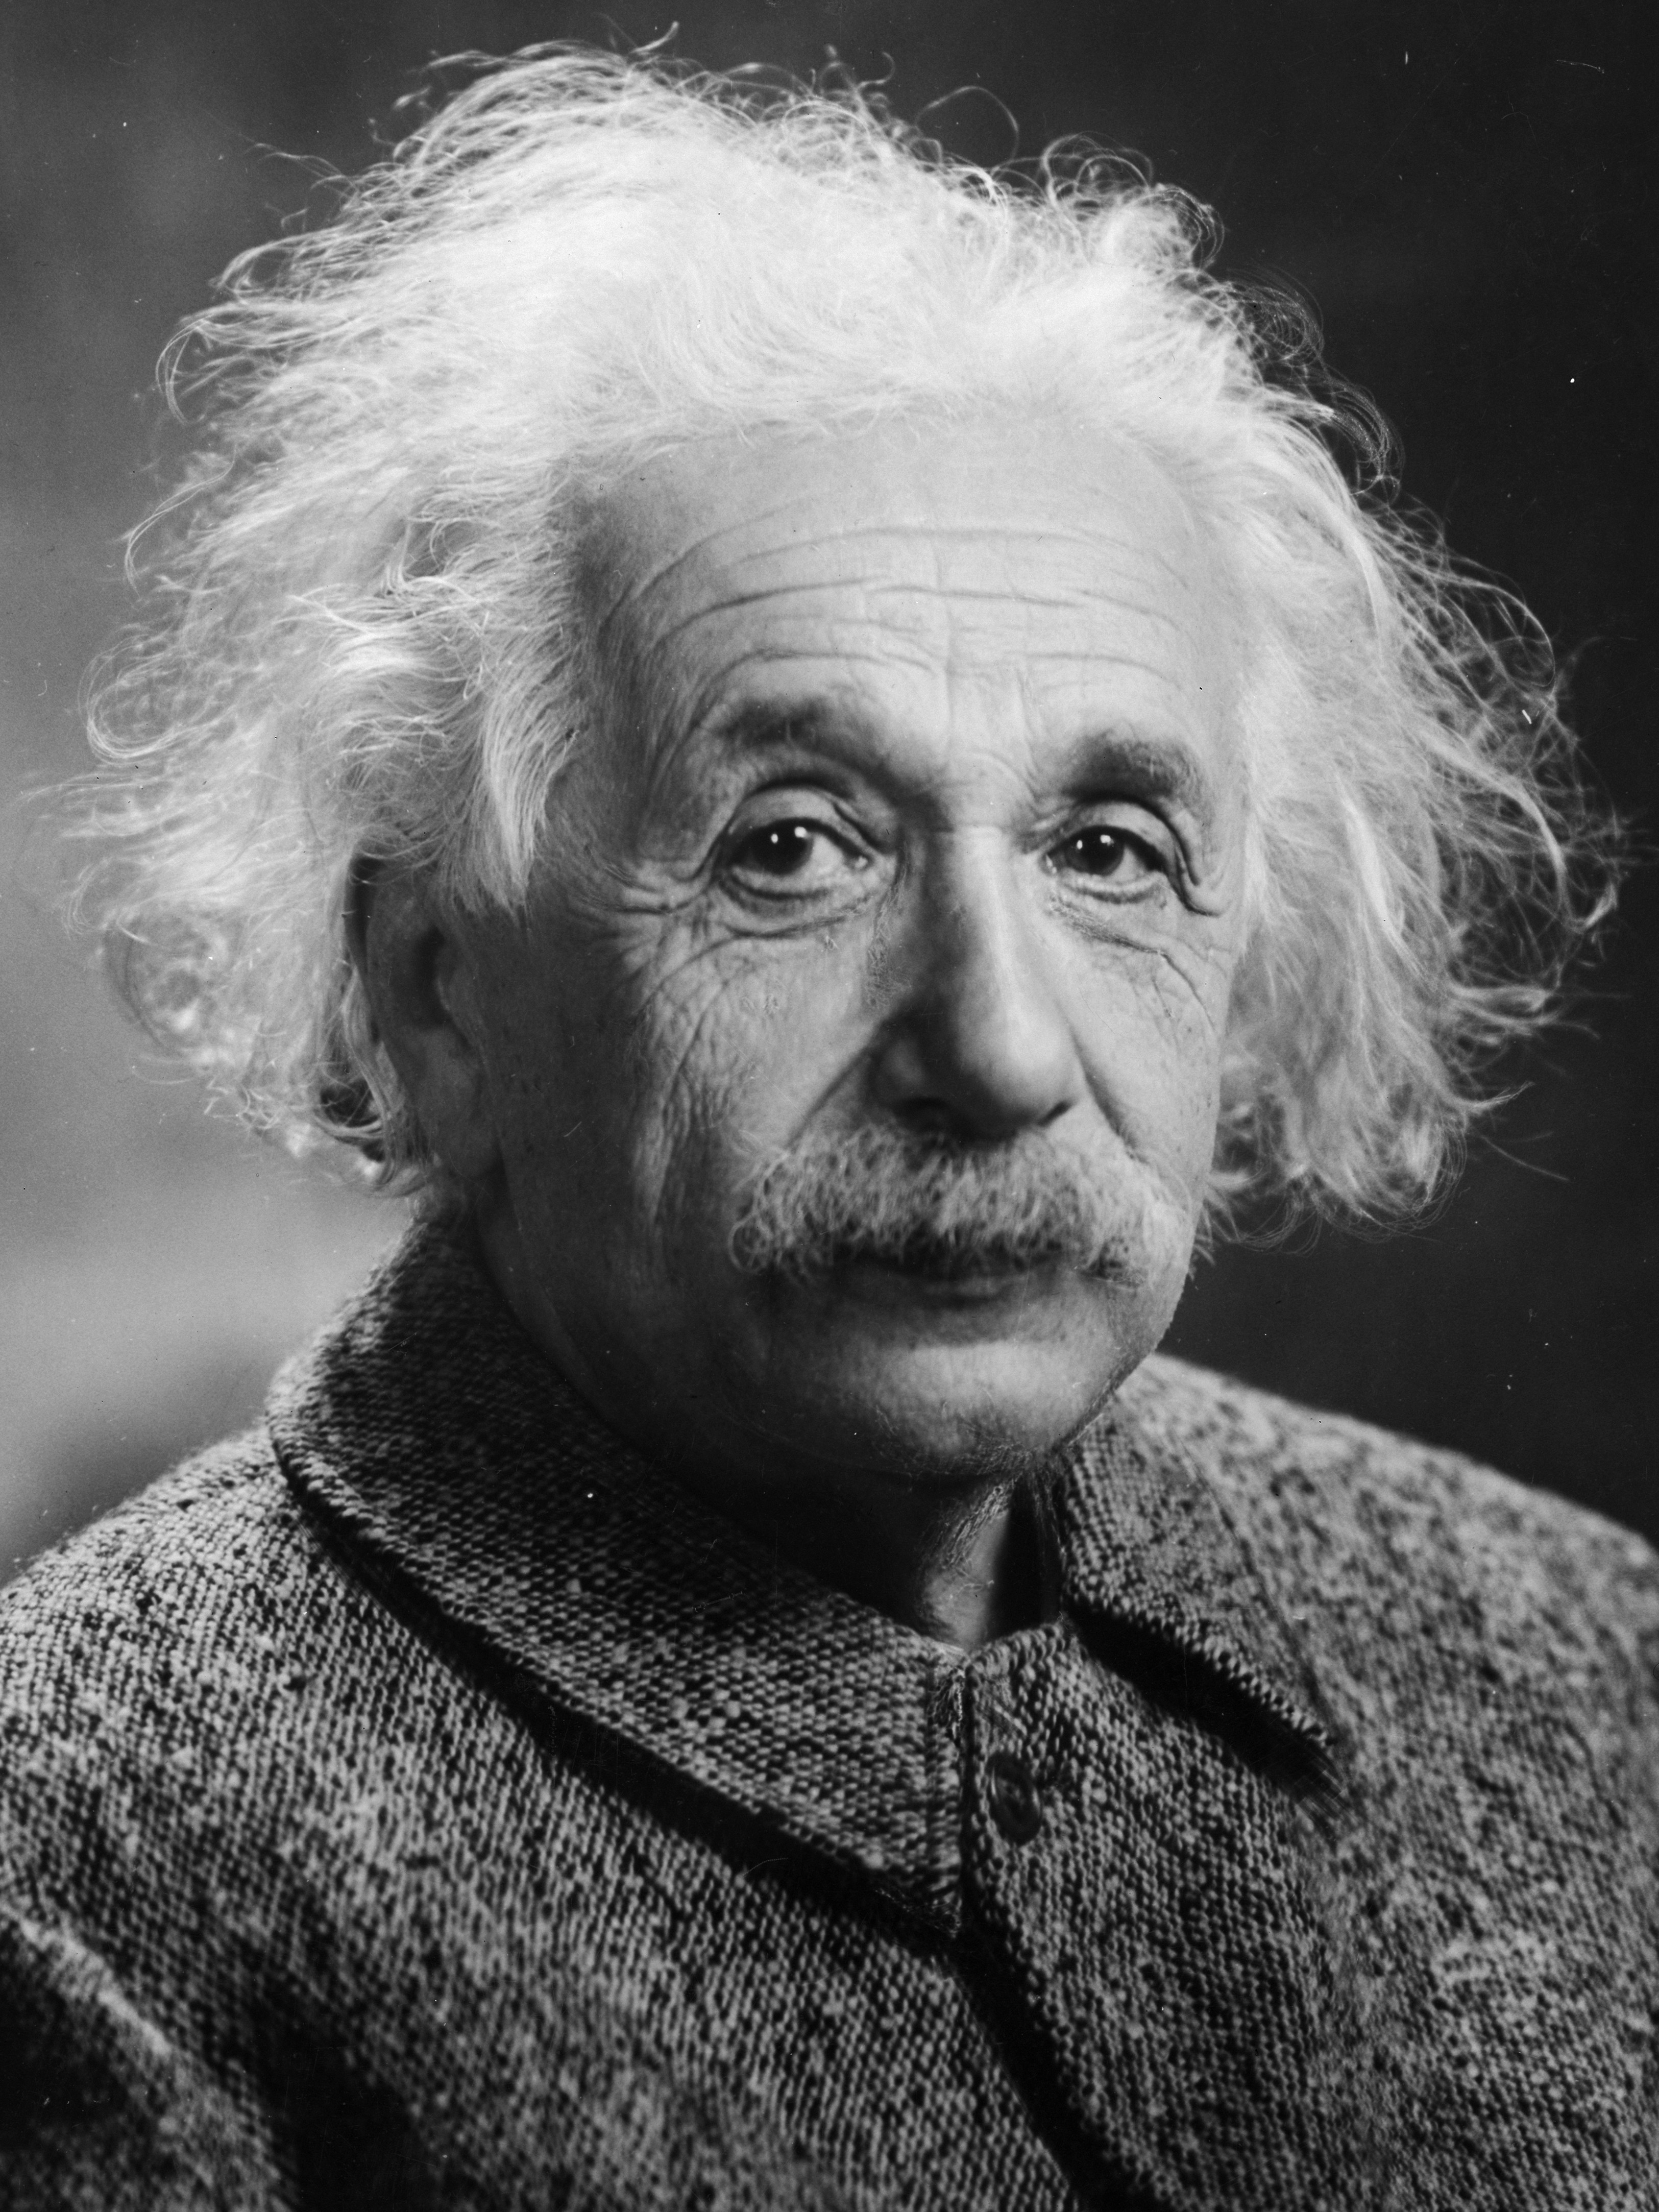
\includegraphics[width=0.8\linewidth]{images/albert-einstein.jpeg}
      Albert~Einstein, speciální~princip~relativity\\\ \\
      \end{center}
  \endminipage\hfill
  \minipage{0.3\textwidth}
  \begin{center}
    \includegraphics[width=0.8\linewidth]{images/erwin-schrödinger.jpg}
        Erwin~Schrödinger, myšlenkový experiment s kočkou v krabici
      \end{center}
  \endminipage\hfill
  \minipage{0.3\textwidth}%
  \begin{center}
    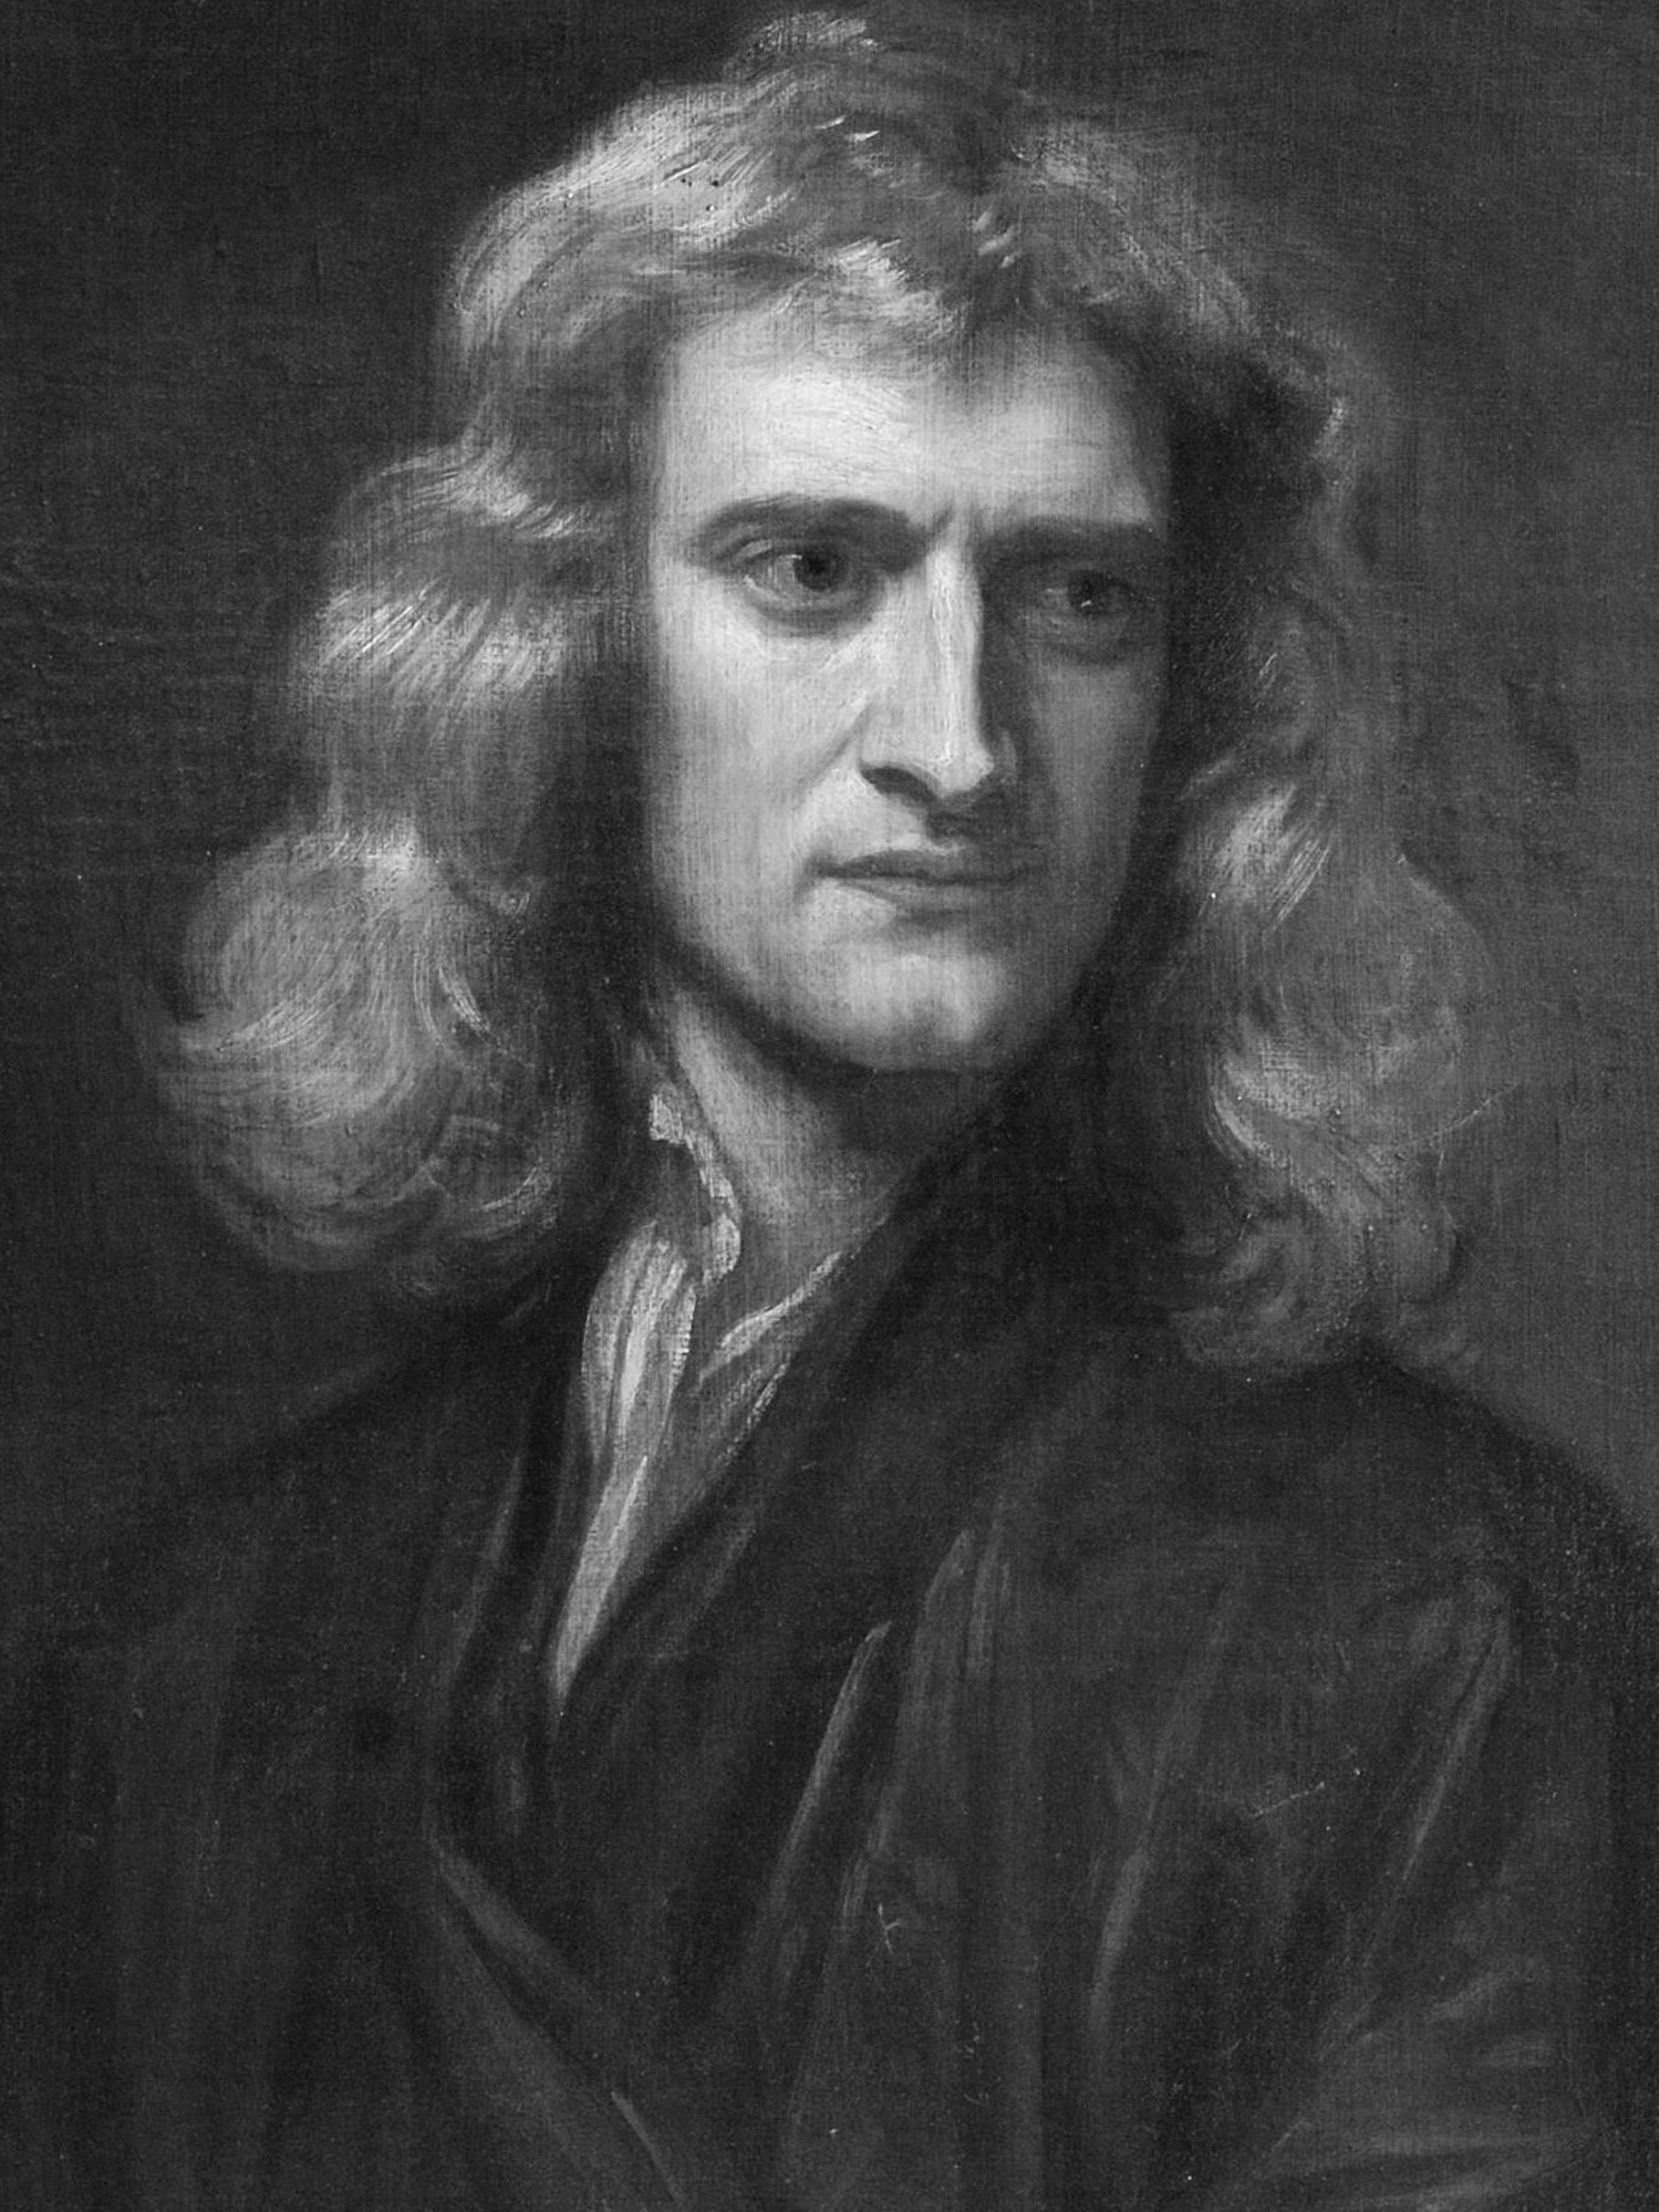
\includegraphics[width=0.8\linewidth]{images/isaac-newton.jpg}
        Isaac~Newton, gravitační~zákon\\\ \\
    \end{center}
  \endminipage
\end{figure}
\vspace{0.5cm}
\begin{figure}[H]
  \minipage{0.3\textwidth}
  \begin{center}
    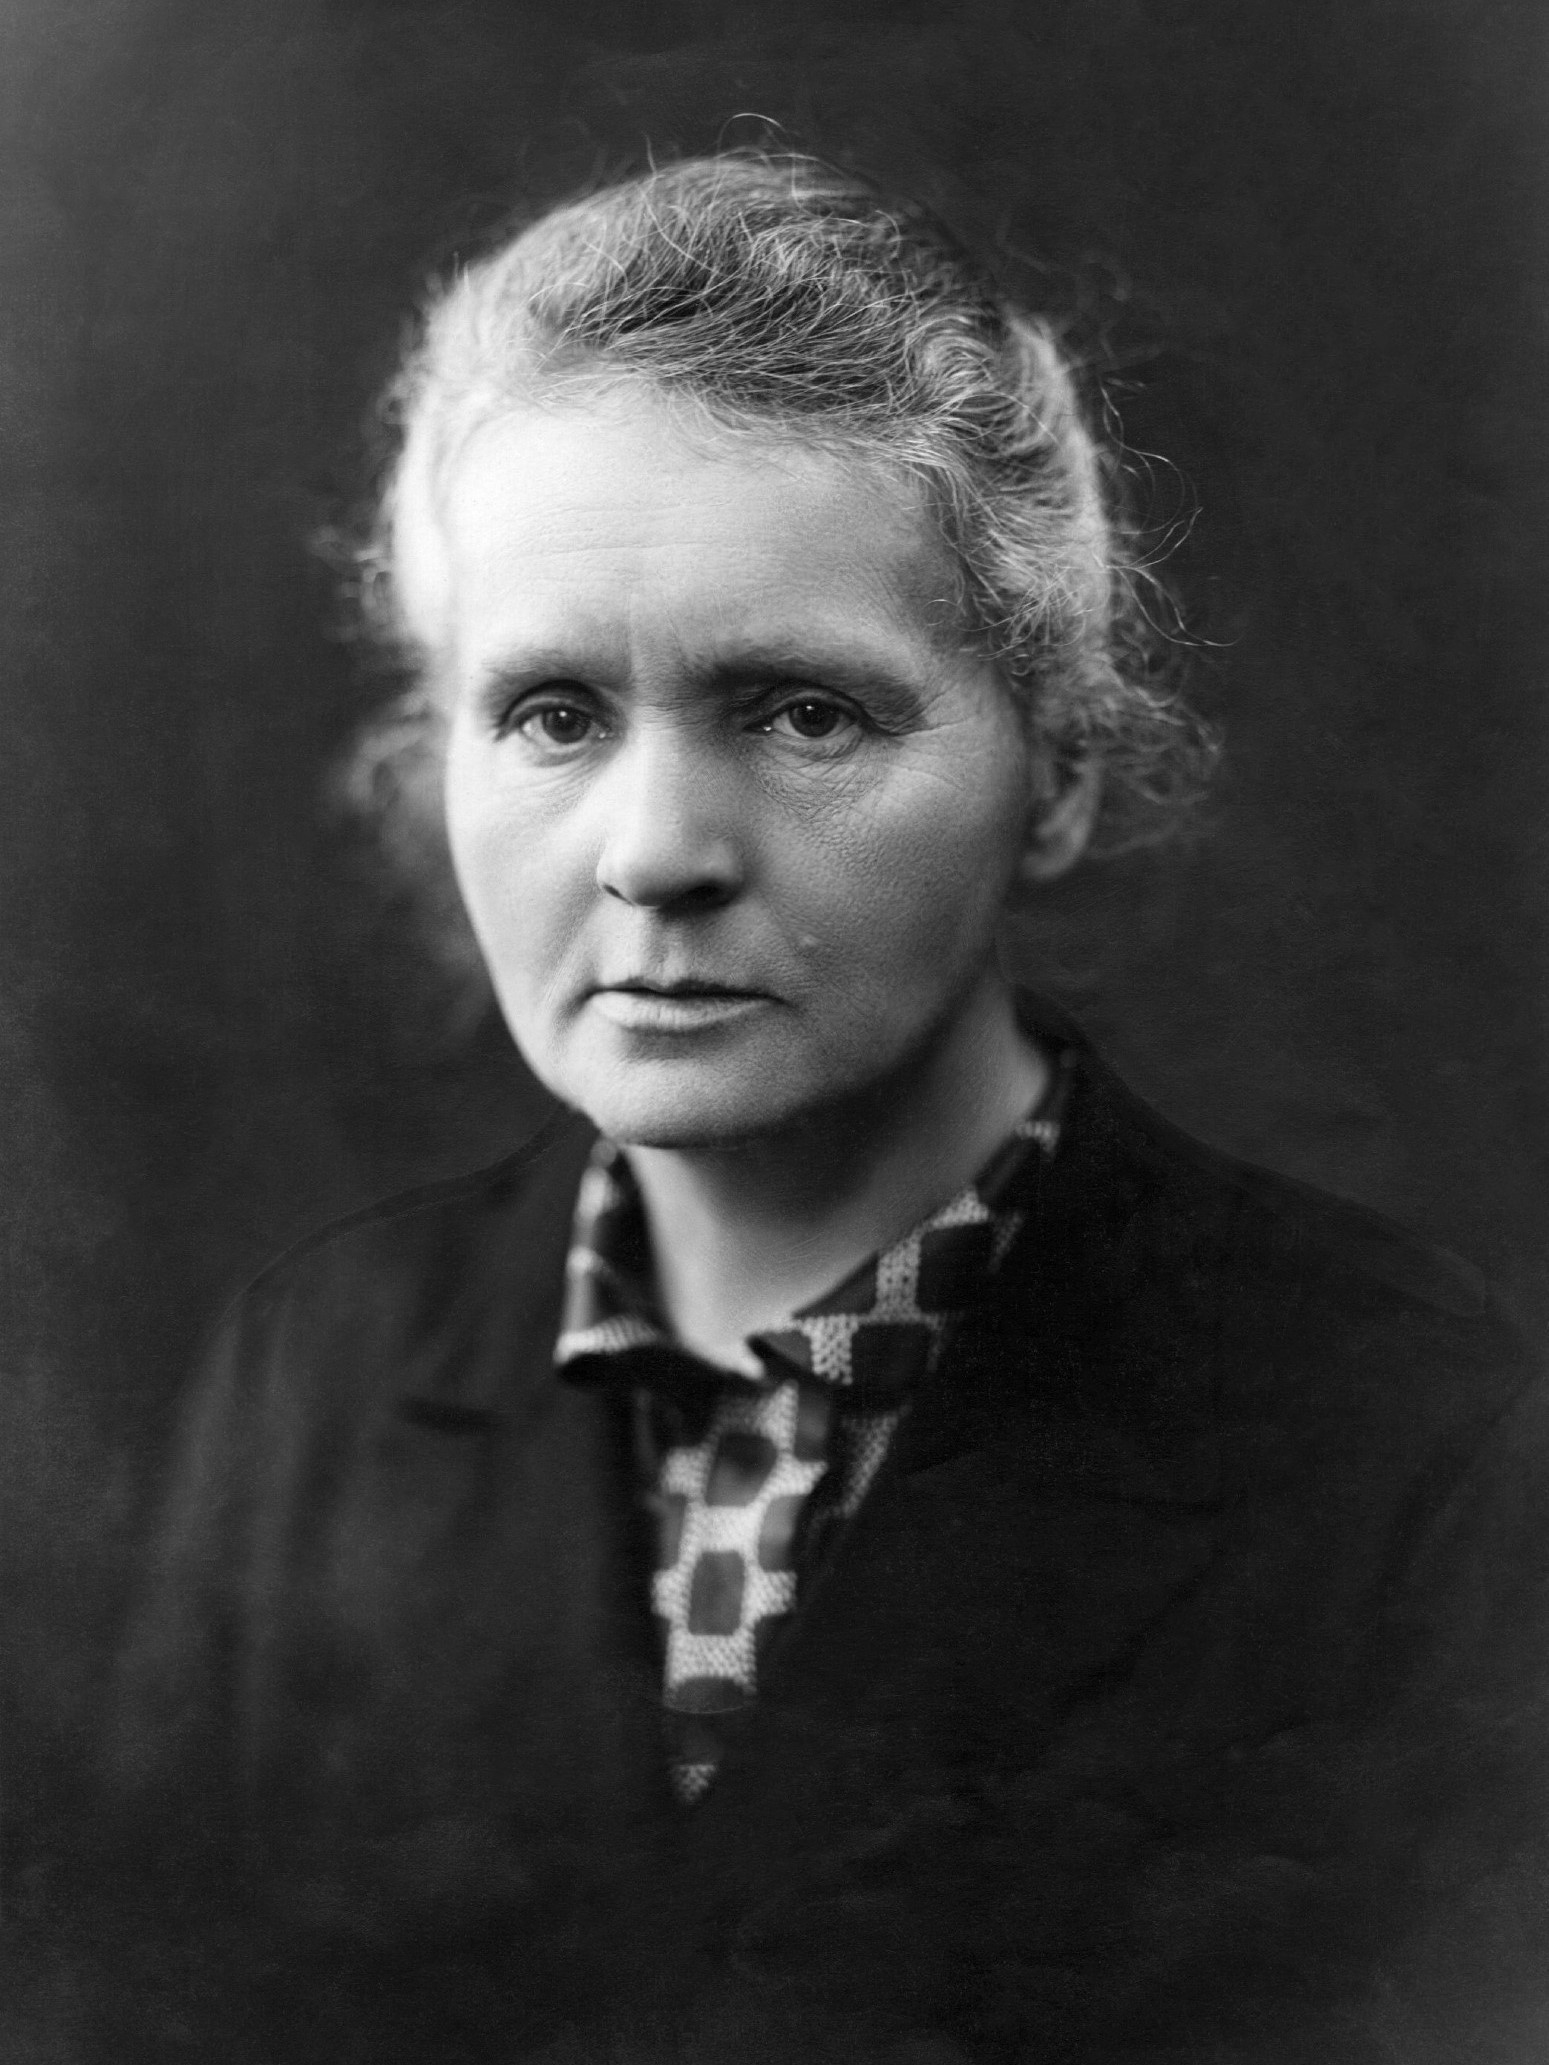
\includegraphics[width=0.8\linewidth]{images/marie-curie-sklodowska.jpg}
        Marie~Curie-Skłodowska, teorie~radioaktivity
      \end{center}
  \endminipage\hfill
  \minipage{0.3\textwidth}
  \begin{center}
    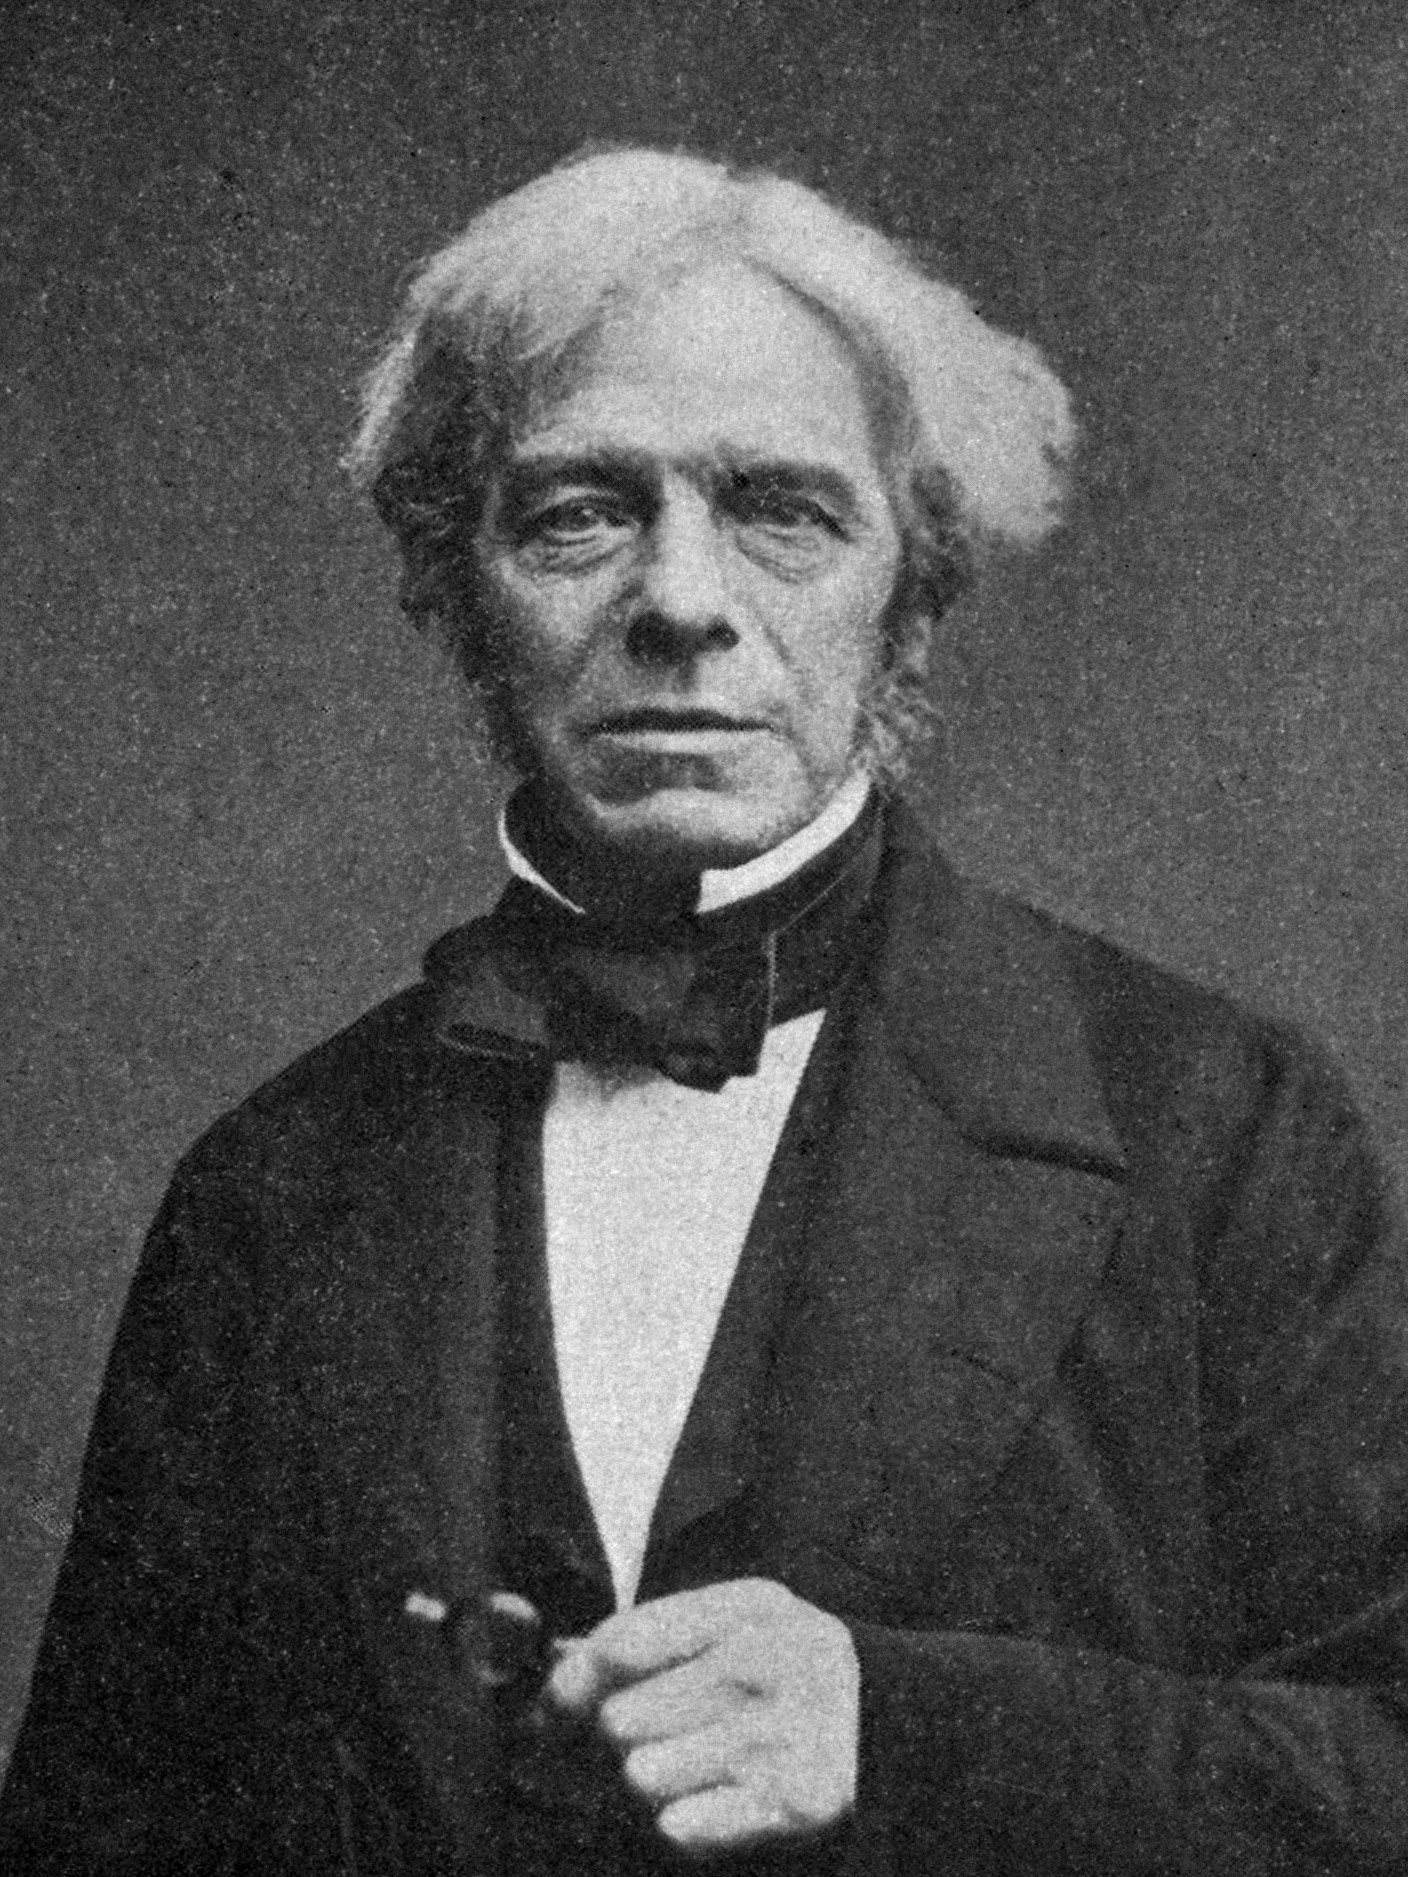
\includegraphics[width=0.8\linewidth]{images/michael-faraday.jpeg}
        Michael~Faraday, elektromagnetická~indukce
      \end{center}
  \endminipage\hfill
  \minipage{0.3\textwidth}
  \begin{center}
    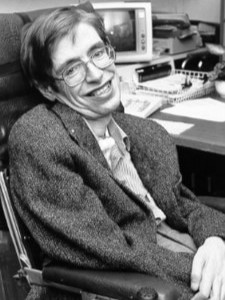
\includegraphics[width=0.8\linewidth]{images/stephen-hawking.jpg}
        Stephen~Hawking, stanovení~teploty~černé~díry
      \end{center}
  \endminipage
\end{figure}
\end{document}
